\documentclass[../../../../main.tex]{subfiles}
\begin{document}

\begin{flushright}
\footnotesize\textit{【自動文字起こし・要確認】}
\end{flushright}

\begin{minipage}[t]{0.5\textwidth}
[解] $\angle \text{BAC} = \angle \text{R}$ となるよう、3頂点 $\text{A}, \text{B}, \text{C}$ を定める。\\
$\text{AB}=c, \text{AC}=b, \text{BC}=a$ となる\\
内接円の中心 $\text{O}$ から各辺に\\
下ろした垂線を $\text{H}_1 \sim \text{H}_3$ と\\
する。題意から\\
$2r + a + b + c = 2 \cdots \text{①}$

(1) $\square \text{AH}_1\text{OH}_3$ が正方形だから、
\[
\begin{cases}
\text{BH}_2 = \text{BH}_1 = c-r \\
\text{CH}_2 = \text{CH}_3 = b-r
\end{cases}
\quad \therefore a = b+c-2r
\]
①に代入して
\[
b+c = 1 \qquad \cdots \text{②}
\]
だから $\quad a = 1-2r$

(2) $\triangle \text{ABC}$ の面積 $S(r)$ とする\\
$S(r) = \frac{1}{2}bc$\\
以下この $\max$ をもとめる。$a, b, c, r > 0$ であり、$\triangle \text{ABC}$ の存在条件から
\[
\begin{cases}
b+c > b+c-2r \\
2b+c-2r > c \\
2c+b-2r > b
\end{cases}
\quad \therefore
\begin{cases}
2r > 0 \\
b-r > 0 \\
c-r > 0
\end{cases}
\]
$A = bc$ とおくと $b, c$ は $t$ の2次方程式 $t^2 - t + A = 0 \ (\because \text{②})$ の\\
$r$ より大なる2実解。判別式 $D$、左辺 $f(t)$ として
\[
\begin{cases}
D \ge 0 \\
f(r) > 0 \\
r < \frac{1}{2}
\end{cases}
\quad \therefore
\begin{cases}
1 - 4A \ge 0 \\
r^2 - r + A > 0 \\
0 < r < \frac{1}{2}
\end{cases}
\]
これを図示すると右図斜線部\\
(境界は $A = \frac{1}{4}$ のみ含む)\\
したがって
\[
\max S(r) = \frac{1}{2} \max A = \frac{1}{8}
\]
\end{minipage}
\begin{minipage}[t]{0.5\textwidth}
\begin{center}
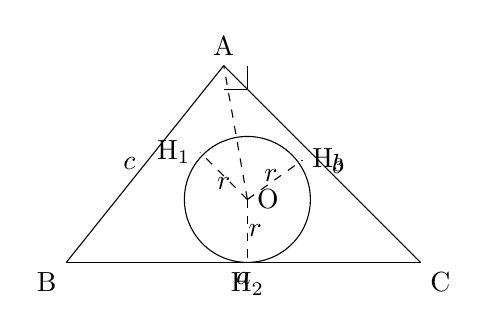
\begin{tikzpicture}
\coordinate (A) at (0, 2.5);
\coordinate (B) at (-2, 0);
\coordinate (C) at (2.5, 0);
\draw (A) -- (B) node[midway, left] {$c$};
\draw (B) -- (C) node[midway, below] {$a$};
\draw (C) -- (A) node[midway, right] {$b$};
\node[above] at (A) {A};
\node[below left] at (B) {B};
\node[below right] at (C) {C};
\draw (A) ++(0,-0.3) -- ++(0.3,0) -- ++(0,0.3);

% Incenter approx
\coordinate (O) at (0.3, 0.8);
\draw (O) circle (0.8);
\node[right] at (O) {O};
\coordinate (H1) at (-0.3, 1.4); % approx on AB
\coordinate (H2) at (0.3, 0); % on BC
\coordinate (H3) at (1, 1.3); % approx on AC

\draw[dashed] (O) -- (A);
\draw[dashed] (O) -- (H1);
\draw[dashed] (O) -- (H2);
\draw[dashed] (O) -- (H3);
\node[left] at (H1) {H$_1$};
\node[below] at (H2) {H$_2$};
\node[right] at (H3) {H$_3$};
\node at (0, 1) {$r$};
\node at (0.6, 1.1) {$r$};
\node at (0.4, 0.4) {$r$};
\end{tikzpicture}
\end{center}

[別] $\cdots a, b$ を消去。完全に\\
内接円と三角形のカンケイから
\[
\frac{1}{2}ab = \frac{1}{2} \cdot r \cdot (2-2r)
\]
\[
ab = 2r(1-r)
\]
(本解)から $a+b=1$ でもあるから $a,b$ は
\[
t^2 - t + 2r(1-r) = 0
\]
の2実解。これが $t > r$ に2実解をもつので
\[
\begin{cases}
r < \frac{1}{2} \\
1 - 8r(1-r) \ge 0 \\
r^2 - r + 2r(1-r) > 0
\end{cases}
\]
$\Rightarrow$ とくと $0 < r \le \frac{2-\sqrt{2}}{4}$ となり、代入してオワリ。

\vspace{1em}
\begin{center}
\begin{tikzpicture}
\draw[->] (-0.5, 0) -- (3, 0) node[right] {$r$};
\draw[->] (0, -0.5) -- (0, 2) node[above] {$A$};
\draw[domain=0:2, smooth, variable=\r] plot ({\r}, {4*(\r/2 - (\r/2)^2)});
\draw (0, 1) -- (2.5, 1);
\node[left] at (0, 1) {$\frac{1}{4}$};
\node[below] at (1, 0) {$\frac{1}{2}$};
\node[right] at (1.5, 0.7) {$A = -r^2+r$};
\fill[pattern=north east lines] (0,0) -- (0,1) -- (1,1) -- plot[domain=1:0] ({\x}, {4*(\x/2 - (\x/2)^2)}) -- cycle;
\end{tikzpicture}
\end{center}
\end{minipage}

\end{document}
